\chapter{Robot User Guide}
\label{app:robotuserguide}
\lhead{Appendix \ref{app:robotuserguide}. \emph{Robot User Guide}}

In this section, the basic operation of the completed \textit{ExplorerBot} robot hardware is outlined. An annotated diagram of the completed robot design is shown in Figure \ref{fig:robotoutlineannotated} below.

\begin{figure}[H]
	\centering
		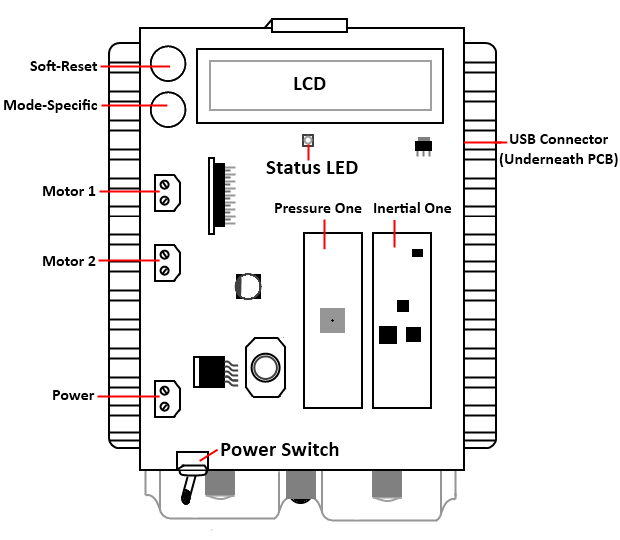
\includegraphics[width=120mm]{RobotOutlineAnnotated.png}
	\rule{35em}{0.5pt}
	\caption[Annotated diagram of the robot]{Annotated diagram of the robot.}
	\label{fig:robotoutlineannotated}
\end{figure}

\section{Power Requirements}

The robot requires a 6-9V DC input power supply, capable of supplying up to 1A of current. Ideally, a 7.2V Lithium Ion battery should be used for this purpose for maximum operating time (due to its ability to supply large amount of instantaneous current, used by the motors when switched on).

\section{Supported USB Devices}

Several classes of USB devices are supported by the robot firmware. Where possible, each class is supported in a generic manner, so that any device compliant with the relevant USB class specification can be used.

\subsection{HID Class Devices}

For robot control over a wired interface, USB HID class devices may be inserted into the robot's USB receptacle. Compatible HID devices must contain at least one four-way directional pad and four buttons for all robot features to be operational. The button mappings are listed in Table \ref{tab:robotbuttonmappings} below.

\begin{table}[H]
	\begin{center}
		\begin{tabular}{ | l | l | l |}
			\hline
			\textbf{Function}		& \textbf{PS3 Controller}	& \textbf{Other HID Device} \\ \hline

			Left					& D-Pad Left				& Button 1	\\ \hline
			Forward					& D-Pad Up					& Button 2	\\ \hline
			Backward				& D-Pad Down				& Button 3	\\ \hline
			Right					& D-Pad Right				& Button 4	\\ \hline
			Headlights (Momentary)	& R2						& Button 8	\\ \hline
			Horn					& L2						& Button 6	\\ \hline
			Headlights (Toggle)		& R1						& Button 7	\\ \hline
			Novelty Horn			& L1						& Button 5	\\ \hline

		\end{tabular}
		\caption[USB HID Robot Button Mappings]{Button mappings between various USB HID devices and the robot functions.}
		\label{tab:robotbuttonmappings}
	\end{center}
\end{table}

In the special case of a Playstation 3 controller being inserted into the robot, the controller will be automatically configured to pair over Bluetooth with the address of the last Bluetooth USB adapter inserted into the robot. Once paired, the controller may then establish a connection with the robot over Bluetooth by pressing the PS3 button located in the center of the controller.

\subsection{Mass Storage Class Devices}

Flash drives suitably formatted with a FAT32 filesystem may be used for sensor logging and system configuration of the robot. Compatible memory sticks must be no more than 4GB in size.

Upon insertion, the robot will attempt to read a file named \texttt{REMADDR.TXT} from the disk. This file should contain the Bluetooth Device Address of the remote device the robot should attempt to establish a connection with while in Bluetooth mode. The format of the stored address is \texttt{XX:XX:XX:XX:XX:XX}, where each \texttt{XX} represents one of the six consecutive octets of the remote device's address in hexadecimal format. If such a file does not exist on the attached disk, a new file is created and populated with the currently stored remote device address.

Also during insertion, a second file called \texttt{SENSLOG.CSV} will be opened. If this file does not exist, a new file is created and populated with the names of the robot's sensors in Comma Separated Values (CSV) format. To begin logging of the robot's sensor data to the attached disk, press the Mode-Specific button next to the LCD.

\subsection{Bluetooth Adapter Devices}

All USB Bluetooth adapters conforming to the Bluetooth 2.1 specification for USB Bluetooth HCI data transport are supported by the robot for Bluetooth mode. When a new adapter device is inserted, the fixed local Bluetooth Address of the adapter is stored into the robot's internal non-volatile EEPROM, for later pairing with any attached Playstation 3 controllers.

To initiate a connection to a remote device, using the address previously store in via a configuration file read from an inserted Mass Storage Device, the Mode-Specific button next to the LCD should be pressed. This will attempt a connection to the stored remote device address, with the connection result being displayed onto the LCD.

All incoming connection and channel requests to the robot will be automatically accepted, however only data carried over the robot's supported services will be processed. Connection and channel information is displayed onto the robot's LCD.

\section{Supported Bluetooth Services}

The robot currently supports three externally exposed services; Service Discovery Protocol, Human Interface Devices, and RFCOMM serial. Other services are not supported and data sent via non-supported services will be ignored by the robot firmware.

\subsection{SDP Service}

The Service Discovery Protocol service is implemented in a Server role only, and is used to expose the remaining services within the robot to external Bluetooth devices during the service discovery phase. All types of server-role requests are supported by the robot.

When requested, the robot will indicate that the device supports the RFCOMM as a server role. This information is used by PCs to automatically allocate and configure a Virtual Serial Port for the robot, used to carry streaming sensor information.

\subsection{HID Service}

The Human Interface Device service is implemented as a client only; the robot accepts reports from external devices, and processes them to determine what actions (if any) must be taken. At present, only three Bluetooth HID devices are supported:

\begin{enumerate}
	\item Sony Playstation 3 controllers,
	\item The Sony-Ericsson z550i mobile phone, and
	\item Nintendo Wii controllers.
\end{enumerate}

With a client implementation of the SDP service, this service could be extended to support Bluetooth HID devices in a generic manner. In the case of the first two supported devices, connections may be established to the robot from the HID device itself. For the Nintendo Wii controller, the connection must be initiated locally from the robot. The robot button mappings for these devices are shown in Table \ref{tab:robotbtbuttonmappings} below.

\begin{table}[H]
	\begin{center}
		\begin{tabular}{ | l | l | l | l | }
			\hline
			\textbf{Function}		& \textbf{PS3 Controller}	& \textbf{z550i Phone}	& \textbf{Wii Controller} \\ \hline

			Left					& D-Pad Left				& Navigation Left		& D-Pad Left	\\ \hline
			Forward					& D-Pad Up					& Navigation Up			& D-Pad Up		\\ \hline
			Backward				& D-Pad Down				& Navigation Down		& D-Pad Down	\\ \hline
			Right					& D-Pad Right				& Navigation Right		& D-Pad Right	\\ \hline
			Headlights (Momentary)	& R2						& Right Button			& Button B		\\ \hline
			Horn					& L2						& Left Button			& Button A		\\ \hline
			Headlights (Toggle)		& R1						& \textit{N/A}			& Button +		\\ \hline
			Novelty Horn			& L1						& \textit{N/A}			& Button -		\\ \hline

		\end{tabular}
		\caption[Bluetooth HID Robot Button Mappings]{Button mappings between the supported Bluetooth HID devices and the robot functions.}
		\label{tab:robotbtbuttonmappings}
	\end{center}
\end{table}

\subsection{RFCOMM Service}

For remote wireless streaming of the robot's sensor data, the RFCOMM wireless Virtual Serial Port service is implemented as a server role. Connecting to the robot via this service using a PC will cause the robot to stream out the current values of the sensors in CSV format. When the virtual serial port connection is first opened, the robot will output the human readable names of each sensor before the sensor values. Only one RFCOMM session may be active at one time.